\documentclass[11pt]{article}

\usepackage[letterpaper, margin=1in]{geometry}

\usepackage[spanish]{babel}
\usepackage[utf8]{inputenc}
\usepackage{multirow}
\usepackage{tabularx}
\usepackage{longtable}



%Figuras
\usepackage{graphicx, subfigure}
\usepackage[]{tikz}
\usepackage{pbox}

%Matemática
\usepackage{amsmath}
\usepackage{amssymb}

%Símbolos mate extra (alfabetos, etc.)
\usepackage{mathrsfs}


%Algoritmos
\usepackage{float}
\usepackage{algorithm}
\usepackage{algorithmicx}
\usepackage{algpseudocode}
\usepackage{listings}


\usepackage{color}
\usepackage{hyperref}

\usepackage{mdframed}
\usepackage{tcolorbox}
\usepackage{multicol}
\usepackage{booktabs}
\usepackage{tabulary}
\definecolor{darkblue}{rgb}{0 , 0.054 , 0.196}



\title{Informe Final Proyecto 1}
\author{Pablo Alfaro Castro - B20162\\Carlos  Jimenez Arroyo - B23397}

\begin{document}

\maketitle
\hrule
\hrule
\tableofcontents
\hspace{5mm}
\hrule
\hrule


\section{Reseña}

 Shearsort es un algoritmo capaz de ordenar una matriz de dimensiones NxN, con la singularidad de que esta queda ordenada en forma serpenteada siendo $N_{0,0}$ el elemento menor, y $N_{N,0}$ el elemento mas grande.
 
\subsection{Estructura}

Teóricamente el algoritmo toma raíz de N veces tiempo para ordenar cada uno de los arreglos, estos ordenamientos suceden periódicamente hasta que un ciclo central se cierre, dentro de este ciclo se ejecutan las instrucciones necesarias para el ordenamiento, este ciclo consta de dos faces:
\begin{itemize}
\item Fase 1: Ejecutar N veces:
\begin{itemize}
\item Ordenar las filas pares de derecha a izquierda, o las impares de izquierda a derecha.
\item ordenar las columnas de arriba hacia abajo.
\end{itemize}
\item Fase 2: Ordenar filas alternando el método anterior.
\end{itemize}


Ordenar una fila de longitud n con la transición par-impar  toma n pasos. Dado que el algoritmo realiza log(n) iteraciones, se requiere nlog(n) pasos para la fila de clasificación más n pasos para la fila adicional de clasificación operación.
En cada iteración, la altura de la zona sin clasificar disminuye en un factor de 2. Esto significa que las columnas contienen una zona sin clasificar de longitud decreciente. Ordenar una columna que contiene una zona no seleccionada de longitud N toma medidas de transiciones tipo par-impar. Por lo tanto, el algoritmo requiere el siguiente numero de pasos:

\begin{equation}
n + \frac{n}{2} + \frac{n}{4} + ... + 2 = 2n - 2
\end{equation}

Donde predomina solamente el n en la ecuación, por lo tanto, si para cada ordenamiento tarda log(n), la complejidad total vendrá dada por O(nlog(n)).

\section{Funcionamiento}

En la figura \ref{fig:1} se muestra el archivo de encabezados de nuestro programa:

\begin{figure}[H]
\centering
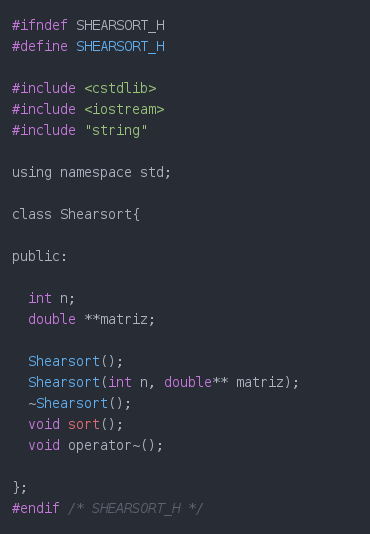
\includegraphics[scale=0.8]{header.png}
\caption{Encabezados}
\label{fig:1}
\end{figure}
\newpage

Se puede ver la estructura básica del algoritmo que se programó, comenzando por el constructor de la clase, así como los atributos y métodos que se listan continuación:

\begin{itemize}
\item public int n: Corresponde al tamaño  de la matriz que se desea ordenar.
\item public double** matriz: Corresponde a la matriz ya armada y en memoria que se quiere ordenar.
\item public void sort(): Este es el método principal que se encarga de realizar todo el ordenamiento y la lógica requerida, es un método vacío ya que todo se trabaja en la matriz que recibe la clase Shearsort().
\item public void operator~(): Este corresponde al operador de impresión de la matriz, que se usó en la matriz antes y después del ordenamiento.
\end{itemize}

En las figuras \ref{fig:2} y \ref{fig:3} se presenta el código que se implementó en el método sort, este método tiene dos variables dentro, que son:
\begin{itemize}
\item int contador: Esta variable esta encargada de almacenar el limite de iteraciones del ciclo central.
\item int temp:  Esta variable se encarga de almacenar temporalmente el numero mayor o menor según sea el caso, para poder hacer los intercambios entre las filas y las columnas.
\end{itemize}

\begin{figure}[H]
\centering
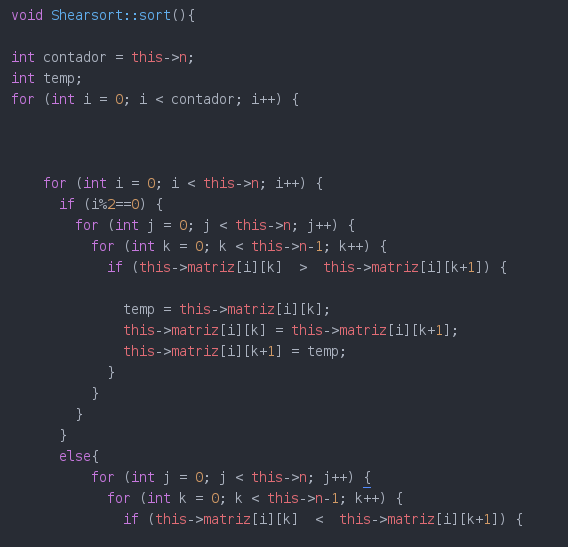
\includegraphics[scale=0.8]{s1.png}
\caption{Shearsot}
\label{fig:2}
\end{figure}

Luego, vienen los ciclos, el ciclo principal, ejecuta los proceso n veces, siendo n el tamaño de la matriz, este limite se determino gracias a ciertos experimentos realizados a mano, seguidamente, dentro de el ciclo central se encuentran los 2 procesos básicos de algoritmo, el ordenamiento de las filas, y el ordenamiento de las columnas, donde cada uno ejecuta un ordenamiento con el método de intercambio de variables.

\begin{figure}[H]
\centering
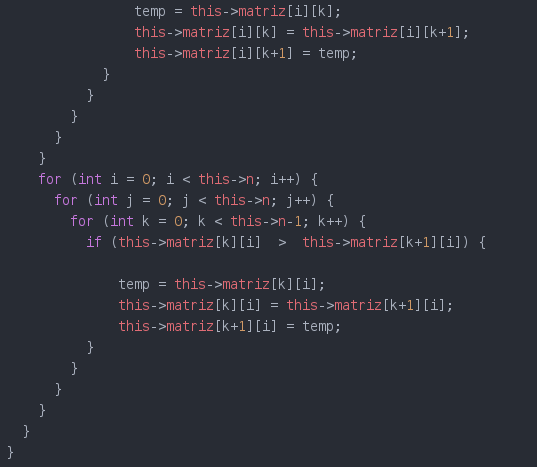
\includegraphics[scale=0.8]{s2.png}
\caption{Shearsort}
\label{fig:3}
\end{figure}

En la figura \ref{fig:4} se muestra el código del operador de impresión, el cual es sencillo, ya que este solo utiliza dos ciclos que van recorriendo toda la matriz, y al final simplemente se imprimió el contenido de esta, uno por uno.

\begin{figure}[H]
\centering
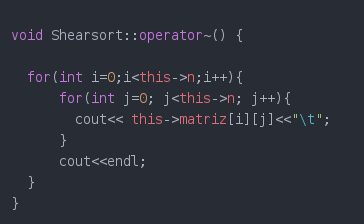
\includegraphics[scale=1]{operator.png}
\caption{Operador de impresión}
\label{fig:4}
\end{figure}

\begin{figure}[H]
\centering
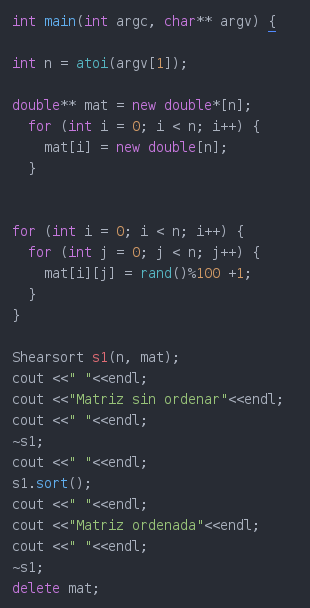
\includegraphics[scale=1]{main.png}
\caption{Main}
\label{fig:5}
\end{figure}

Por ultimo, la figura \ref{fig:5} muestra el código del main, en el cual podemos ver como desde ahí se construyo un objeto de la clase matriz, con atributo n establecido por el usuario y una matriz generada aleatoriamente como se muestra en la imagen, de ese modo se asignó memoria para la matriz, ya por ultimo, se muestra la llamada al método sort, y el operador de impresión antes y después de ordenada la matriz.

\section{Experimentos Realizados}

Para determinar la condición de parada del ciclo central del algoritmo, se realizaron pruebas escritas y hechas a mano, probando el algoritmo con matrices de pequeño tamaño, así se pudieron contar las veces que se repetía el ciclo para de esta manera determinar un patrón de repetición, el cual se encontró por estos medios, de modo que si se contaban los ciclos individualmente (tanto columnas y filas), se requería 2N - 1 ciclos para poder realizar el ordenamiento, debido a que en la manera que se programó el código los ciclos se ejecutan doblemente (en conjunto fila y columna) el numero de culos se vería reducido a la mitad, dejando el limite como N, ya que hablar de medio ciclo no es una posibilidad en este caso.

Para realizar los experimentos y pruebas se utilizaron 2 computadores portátiles, una computadora personal con sistema operativo Debian, 6GB de RAM, Procesador Core i5, y una máquina con el sistema operativo Ubuntu instalado en una máquina virtual, con 2 GB de RAM y un procesador intel core i7, asimismo se decidió por llenar las matrices de forma aleatoria con números del 1 al 100, y que el usuario sea quien determine las dimensiones de la matriz a ordenar. Se realizaron varias pruebas midiendo el tiempo del sistema en ejecutar lo solicitado aumentando la dimensión de la matriz empezando en 2 elevado a la 1 y aumentando el exponente en una unidad.  

\section{Resultados Obtenidos}
De acuerdo a los experimentos realizados poniendo a prueba el código escrito en el lenguaje de C++ para implementar el algoritmo Shearsort, se realizaron pruebas hasta que el tiempo de respuesta del programa se elevó hasta el punto que el programa no imprime una respuesta y se queda "colgado". Como se mencionó antes, al ir aumentando las dimensiones de la matriz en potencias de 2, se lograron obtener 8 muestras con tiempos constantes, A continuación se muestran capturas de pantalla del programa trabajando en las 8 diferentes pruebas realizadas.

\begin{figure}[H]
\centering
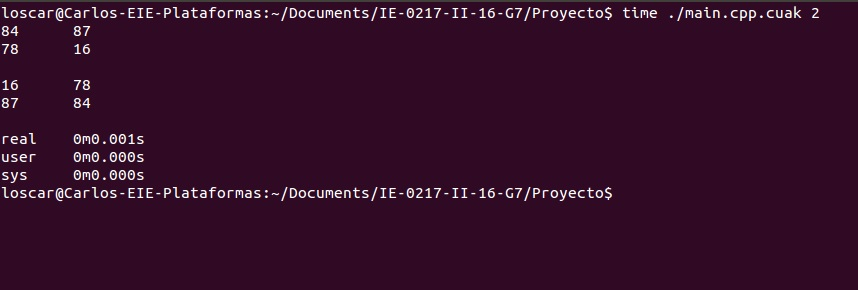
\includegraphics[scale=1]{2x2.jpg}
\caption{Para una matriz 2x2}
\label{fig:6}
\end{figure}

\begin{figure}[H]
\centering
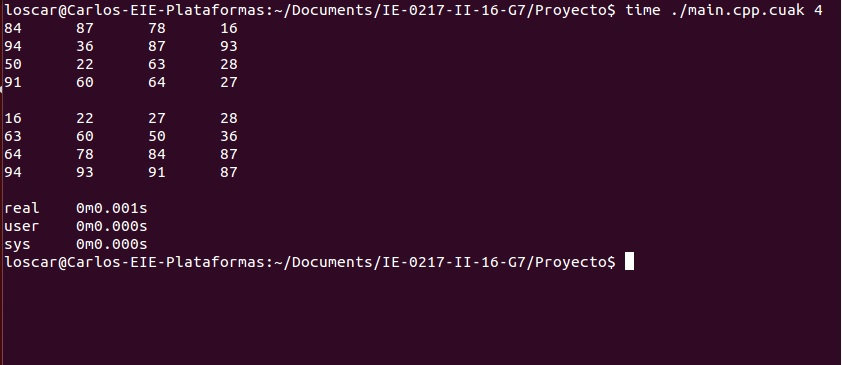
\includegraphics[scale=1]{4x4.jpg}
\caption{Para una matriz 4x4}
\label{fig:7}
\end{figure}

\begin{figure}[H]
\centering
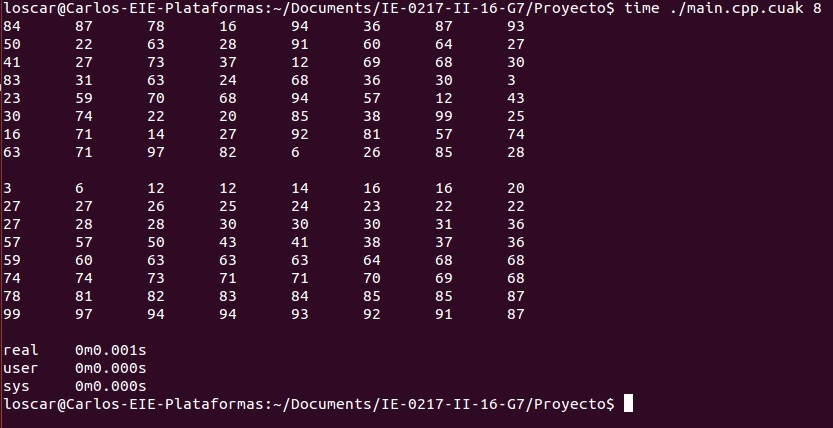
\includegraphics[scale=1]{8x8.jpg}
\caption{Para una matriz 8x8}
\label{fig:8}
\end{figure}

\begin{figure}[H]
\centering
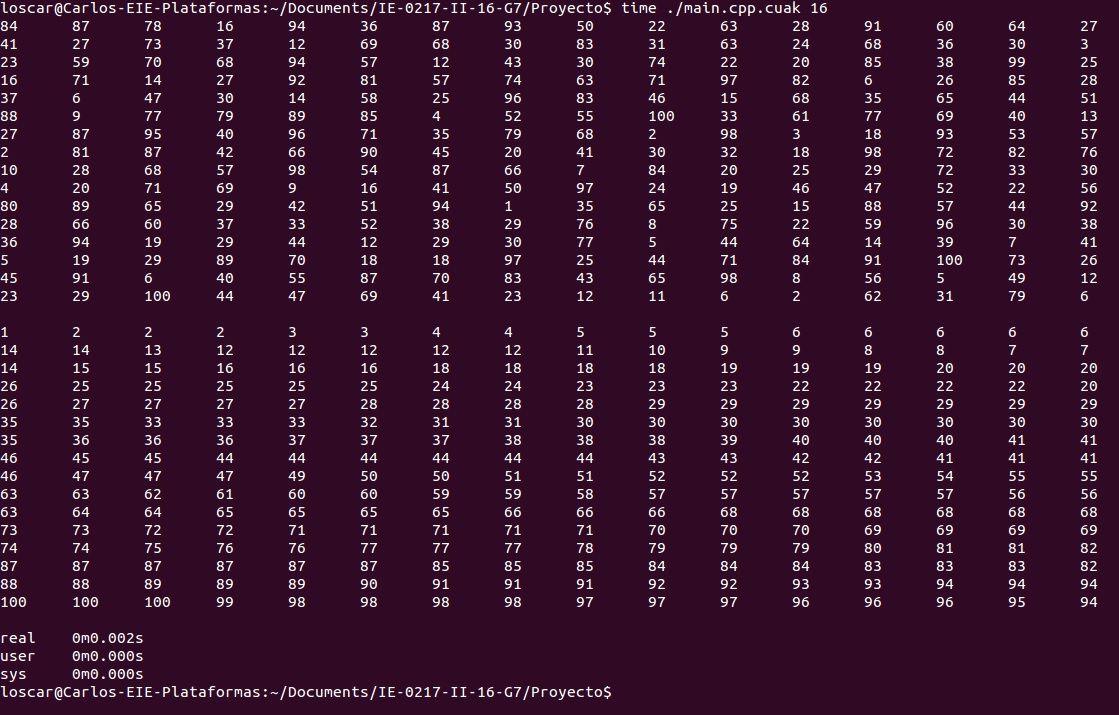
\includegraphics[scale=0.75]{16x16}
\caption{Para una matriz 16x16}
\label{fig:9}
\end{figure}

\begin{figure}[H]
\centering
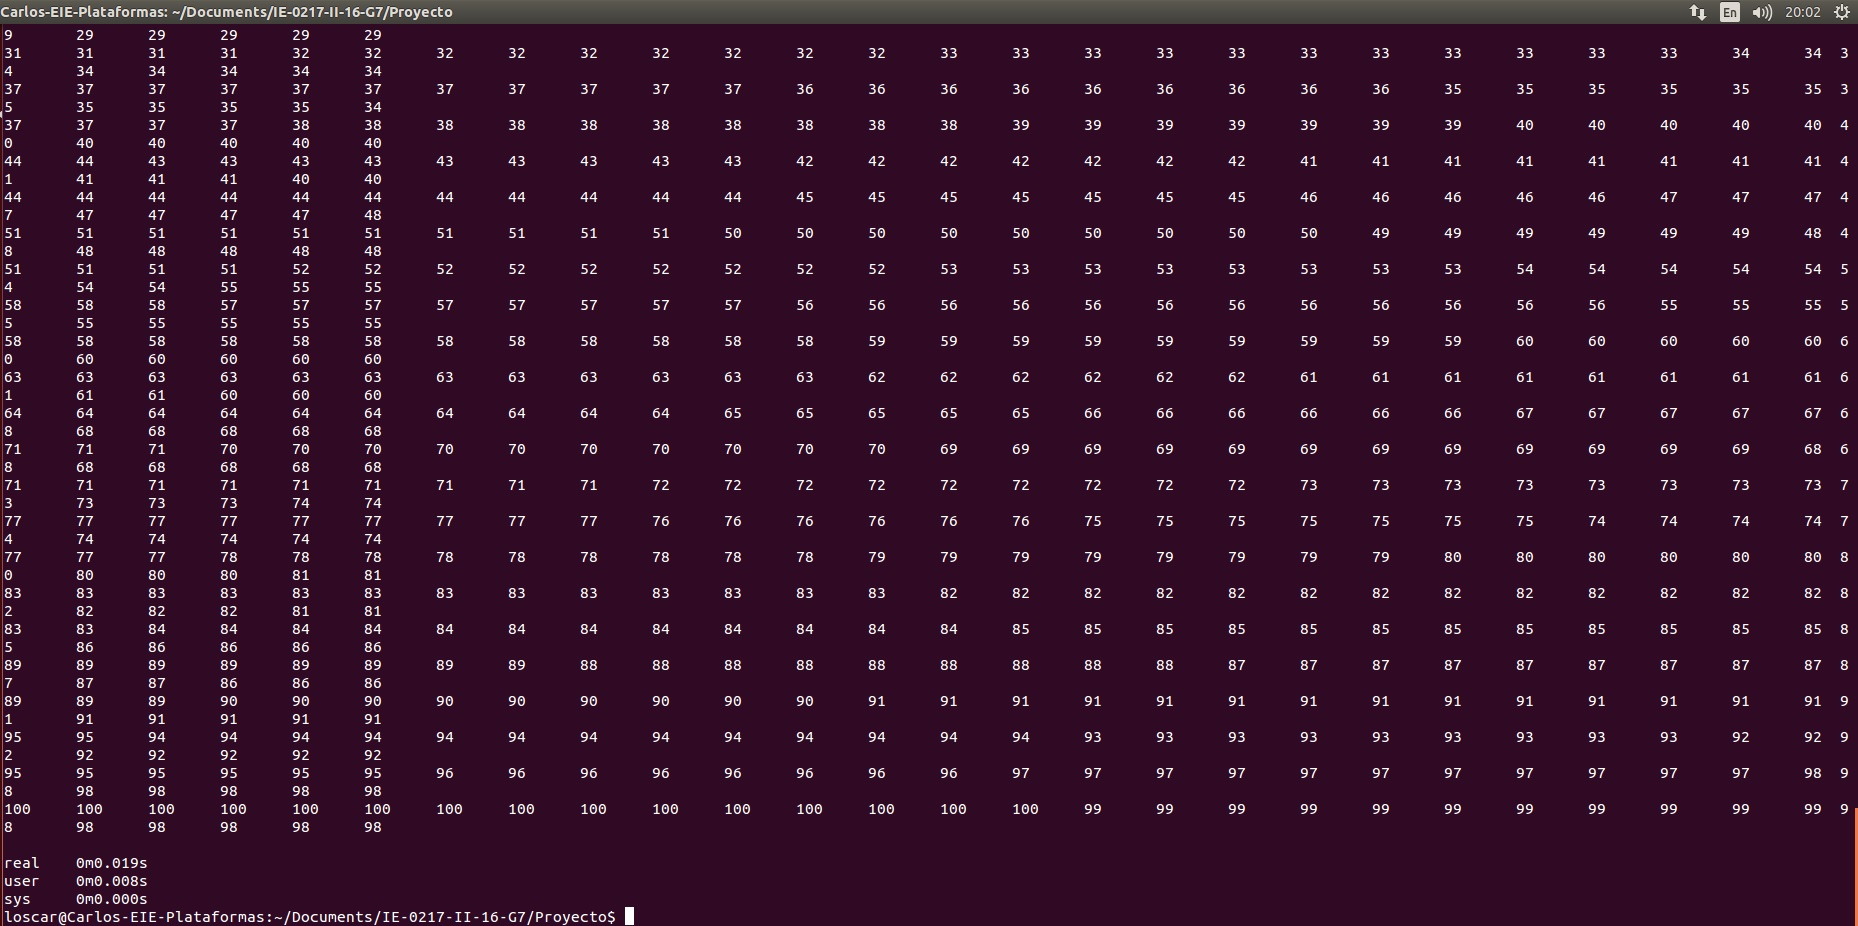
\includegraphics[scale=0.5]{32x32.jpg}
\caption{Para una matriz 32x32}
\label{fig:10}
\end{figure}

\begin{figure}[H]
\centering
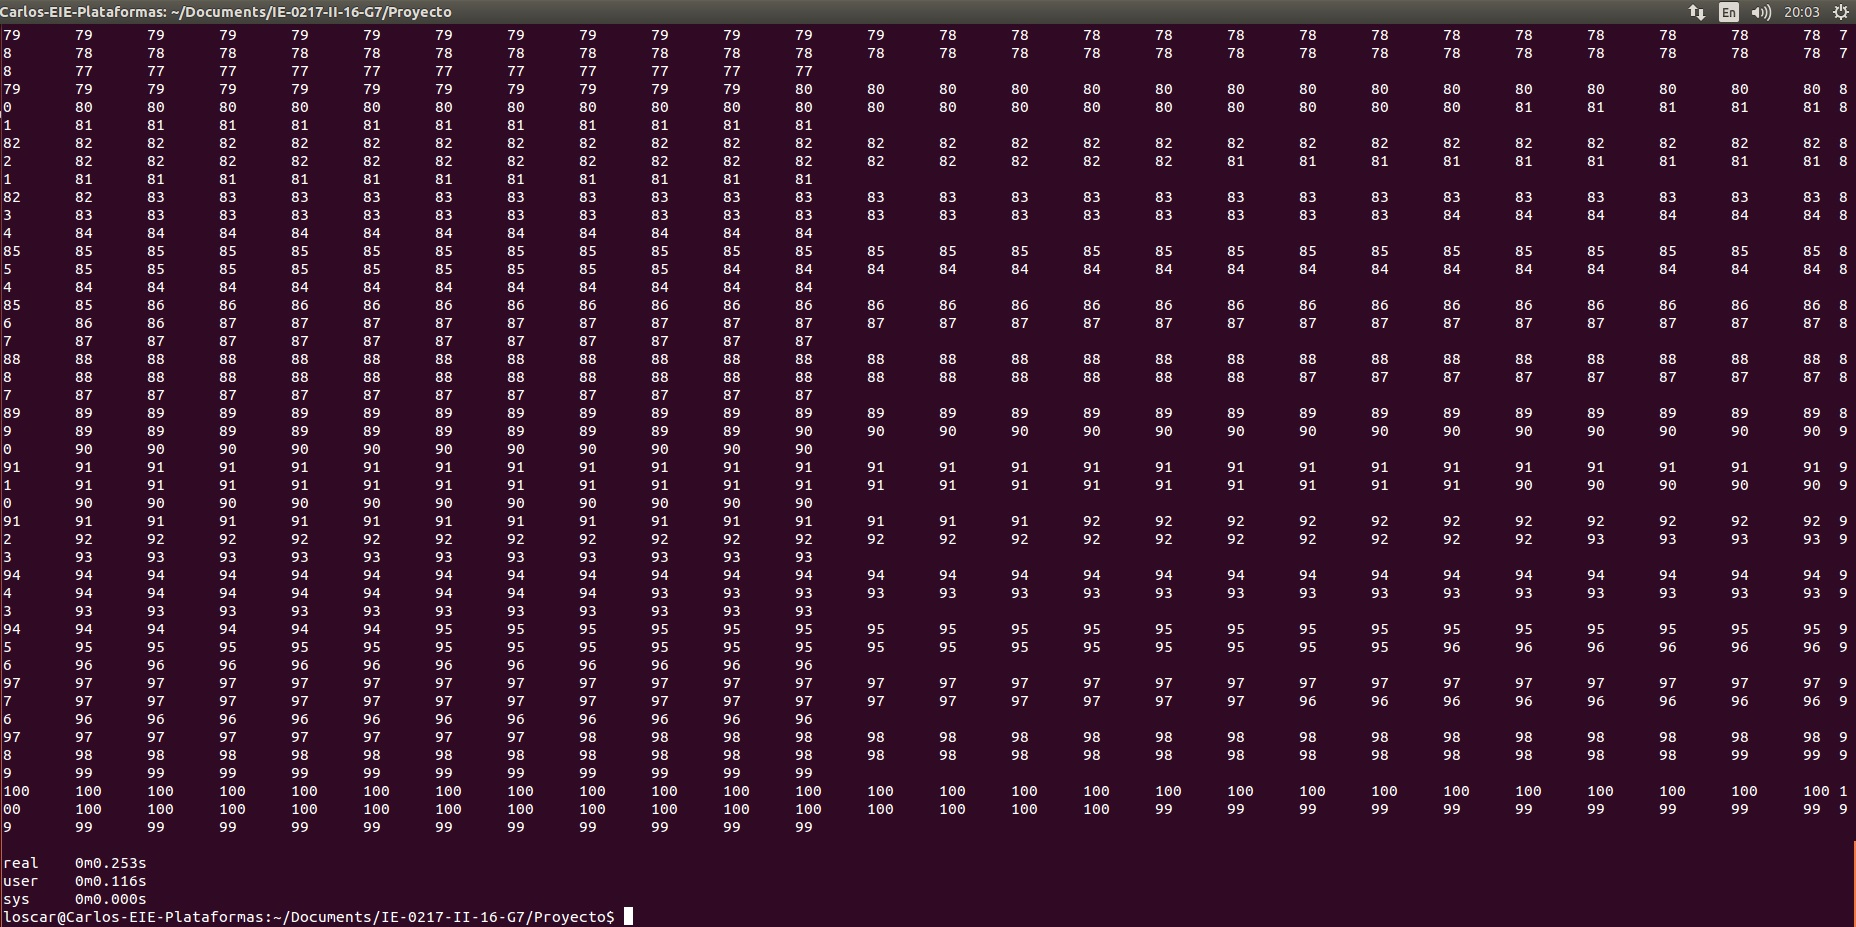
\includegraphics[scale=0.5]{64x64.jpg}
\caption{Para una matriz 64x64}
\label{fig:11}
\end{figure}

\begin{figure}[H]
\centering
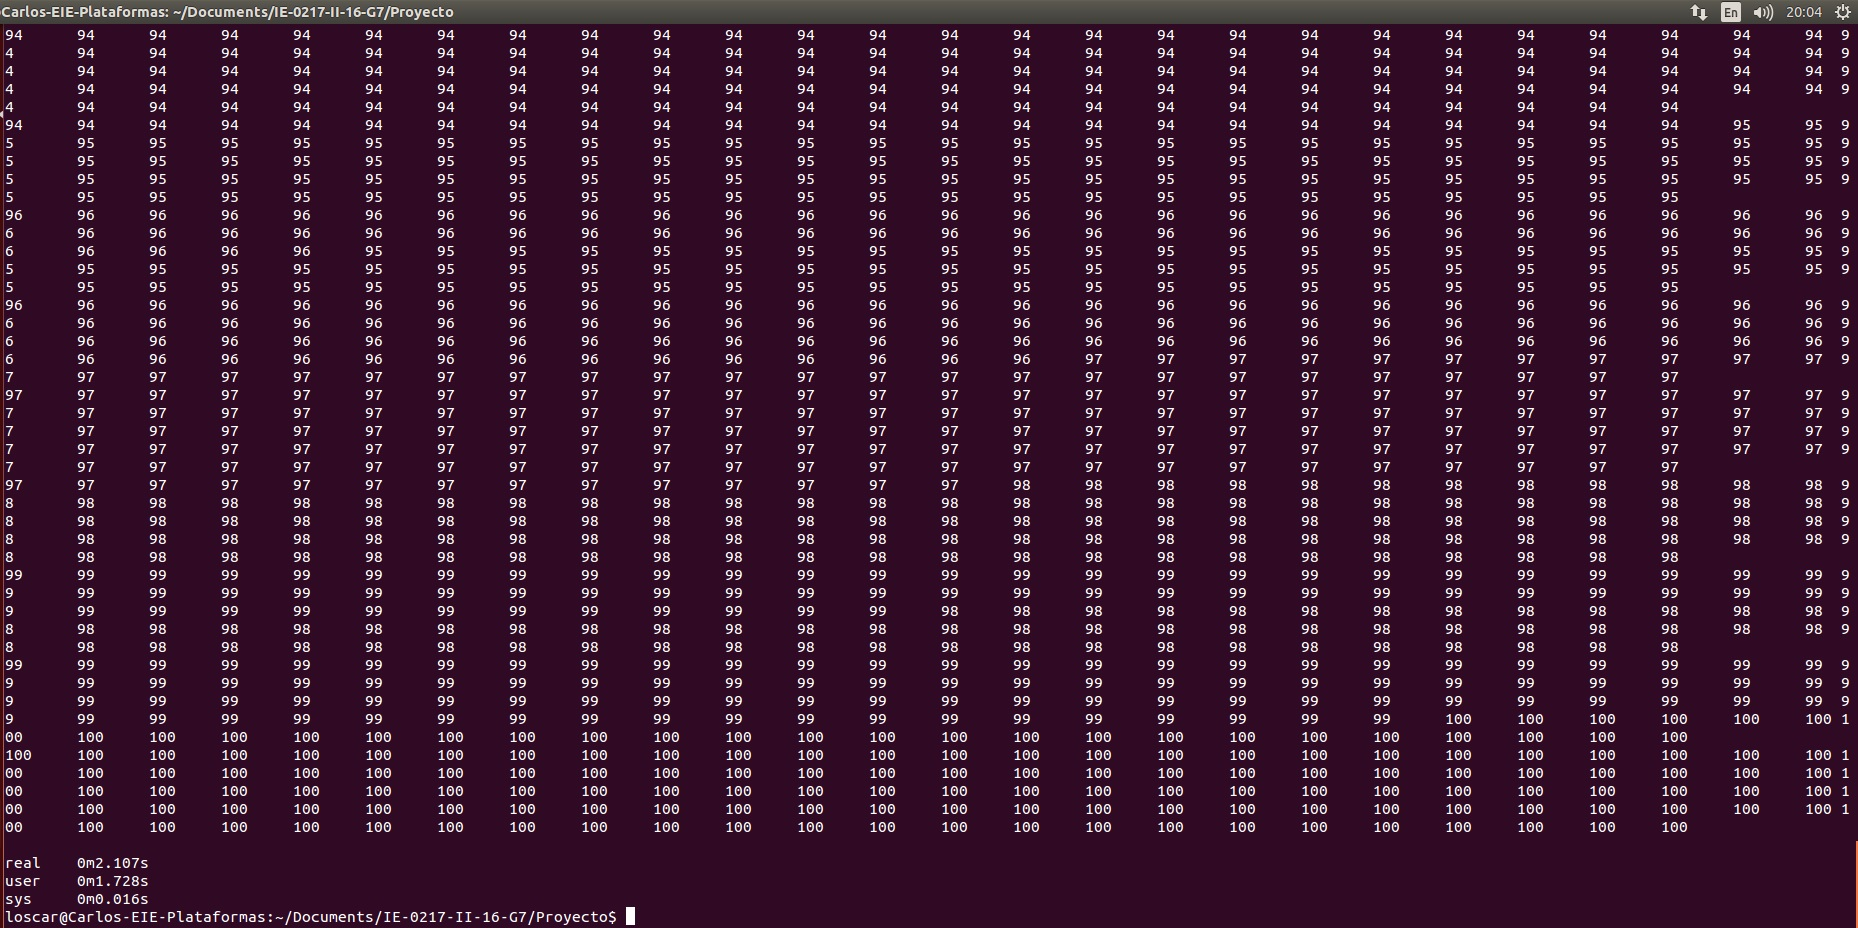
\includegraphics[scale=0.5]{128x128.jpg}
\caption{Para una matriz 128x128}
\label{fig:12}
\end{figure}

\begin{figure}[H]
\centering
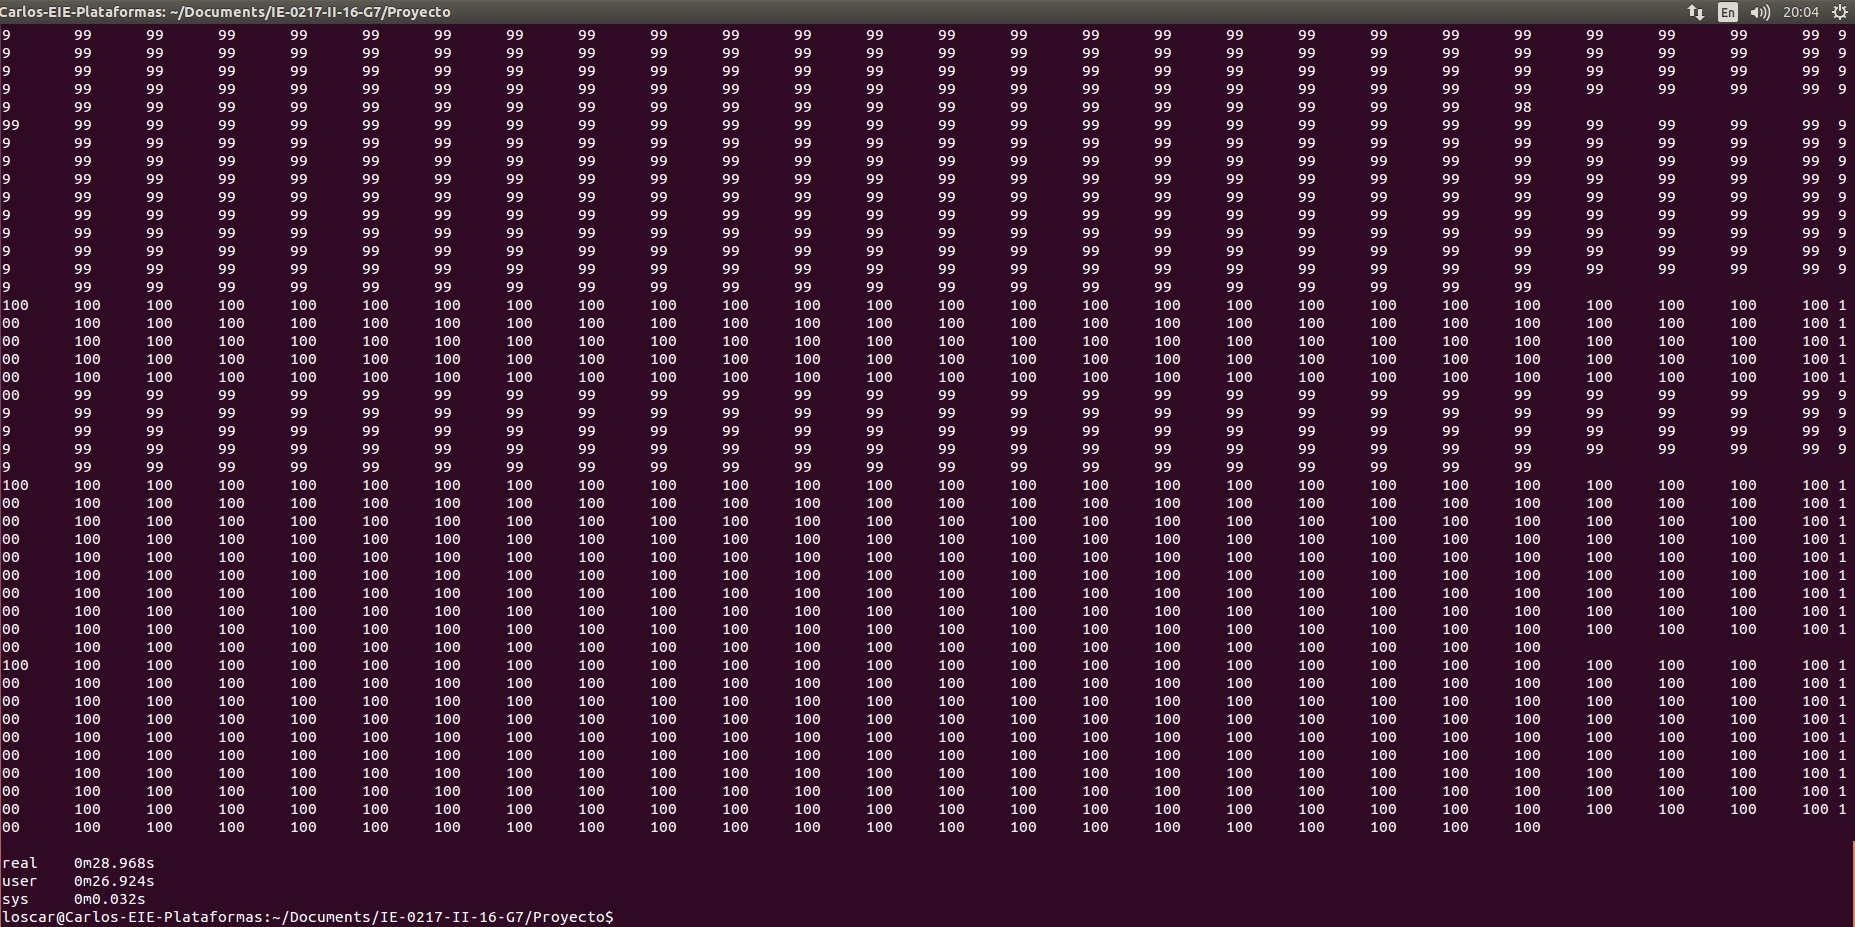
\includegraphics[scale=0.5]{256x256.jpg}
\caption{Para una matriz 256x256}
\label{fig:13}
\end{figure}

Así como se puede apreciar en las capturas de pantalla del programa mostradas, el tiempo que se toma para verificar el funcionamiento correcto del programa corresponde al tiempo mostrado como "real" en las 8 figuras anteriores. Se decidió realizar la prueba varias veces para cada una de las 8 dimensiones que el programa logró manejar, a continuación se presenta una tabla que muestra el tiempo promedio en segundos que el programa duró en ordenar las matrices, estos promedios se sacaron luego de realizar 8 pruebas por cada dimensión de matriz. 

\begin{table}[H]
\centering
\begin{tabular}{p{5cm} p{8cm}}
\hline
Dimensión de la Matriz & Duración registrada del algoritmo \\
\hline \hline
Matriz de tamaño 2x2. & 0.001 segundos \\
\hline
Matriz de tamaño 4x4. & 0.001 segundos\\
\hline
Matriz de tamaño 8x8. & 0.001 segundos\\
\hline
Matriz de tamaño 16x16. & 0.002 segundos\\ 
\hline
Matriz de tamaño 32x32. & 0.017 segundos\\ 
\hline
Matriz de tamaño 64x64. & 0.168 segundos\\ 
\hline
Matriz de tamaño 128x128. & 1.917 segundos\\ 
\hline
Matriz de tamaño 256x256. & 28.023 segundos\\ 
\hline
\end{tabular}+
\label{tabla:Tiempos}
\end{table}

De esta forma vemos como el tiempo que requiere el programa para poder trabajar se aumenta considerablemente a partir de la dimensión 256x256, hasta el punto que que no se pudo obtener una muestra de tiempo para un arreglo de tamaño 512x512.



\section{Análisis de tiempos de ejecución y complejidad computacional}

Teóricamente se sabe que el algoritmo Shearsort puede llegar a poseer complejidad de: \begin{equation}
\sqrt[]{n}*log(n)
\end{equation}Esto en el peor de los casos, sin embargo, en la implementación hecha en el experimento realizado se tiene un comportamiento más parecido a una complejidad de: \begin{equation}
n*log(n)
\end{equation}

Dicha complejidad también puede presentarse en algunos casos de este algoritmo. 

\begin{figure}[H]
\centering
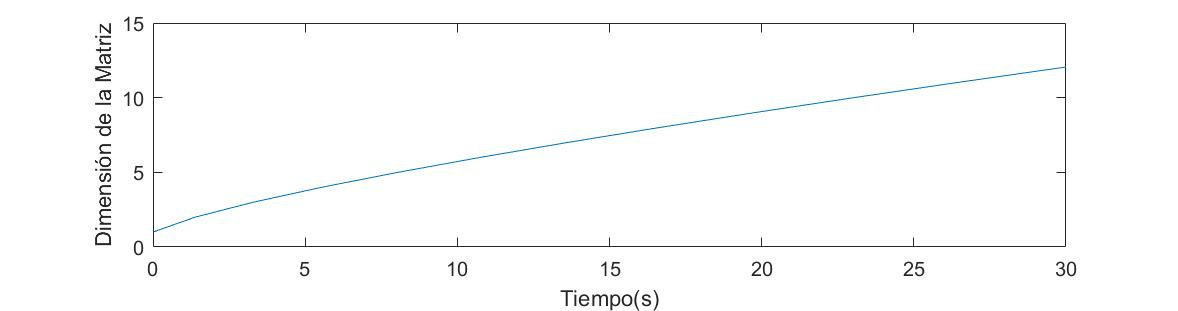
\includegraphics[scale=0.5]{gr_fica_complejidad.jpg}
\caption{Gráfica para la complejidad nlog(n).}
\label{fig:14}
\end{figure}

Como se puede ver en la figura \ref{fig:14}, la gráfica corresponde a la representación gráfica de la complejidad de la nlog(n).

\begin{figure}[H]
\centering
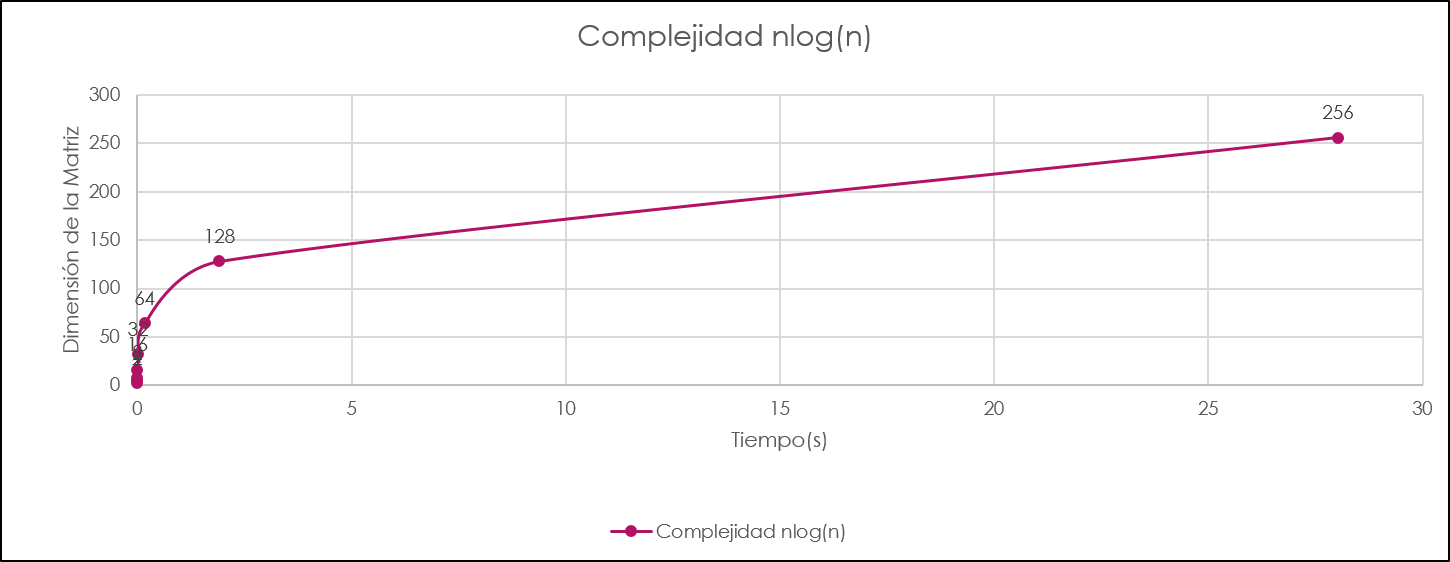
\includegraphics[scale=0.5]{grafica.png}
\caption{Gráfica obtenida en durante la experimentación.}
\label{fig:15}
\end{figure}

 En la figura \ref{fig:15} tenemos la gráfica que se obtuvo con los tiempos promediados de trabajo del programa, como se puede ver, existe un comportamiento similar con la gráfica presentada en la figura \ref{fig:14}. El hecho de que el comportamiento no sea exactamente igual al teórico puede venir de la mano de ya sea por elementos de hardware o software, por ejemplo, podría afectar el hecho de que las pruebas se realizaran en una máquina virtual, lo cual pudo limitar un poco el funcionamiento del programa de alguna u otra forma, no obstante el comportamiento obtenido es bastante aceptable cuando comparamos la reacción obtenida con la teórica.

\section{Conclusiones}

\begin{itemize}
\item Se logró construir un programa en C++ que generara un ordenamiento de un arreglo de tamaño nxn de la forma que lo hace el algoritmo Shearsort.
\item Se comprobó experimentalmente que la función de tiempo generada de acuerdo a las pruebas realizadas al programa cumplen con la forma de la función de complejidad teórica del algoritmo.

\end{itemize}

\section{Bibliografía}

\begin{itemize}

\bibliography{ref}


\item Parallel Sorting Algorithms (s. f.). Recuperado de http://www.cpp.edu/~gsyoung/CS370/14Sp/Parallel%20Sorting%20Algorithms%20Matthew.pdf

\item Tomey, M. Á. (13 de Octubre de 2016).Algoritmos de Ordenación Paralelos

\item Shearsort (s. f.). Recuperado el 23 de Octubre del 2016, de https://www.cse.iitb.ac.in/~ranade/606/shearsort.pdf

\end{itemize}

\section{Anexos}

\subsection{main.cpp}

\begin{lstlisting}
#include "shearsort.h"
#include "cstdlib"




int main(int argc, char** argv) {

int n = atoi(argv[1]);

double** mat = new double*[n];
	for (int i = 0; i < n; i++) {
		mat[i] = new double[n];
	}


for (int i = 0; i < n; i++) {
  for (int j = 0; j < n; j++) {
    mat[i][j] = rand()%100 +1;
  }
}

Shearsort s1(n, mat);

cout <<" "<<endl;
cout <<"Matriz sin ordenar"<<endl;
cout <<" "<<endl;
~s1;
cout <<" "<<endl;
s1.sort();
cout <<" "<<endl;
cout <<"Matriz ordenada"<<endl;
cout <<" "<<endl;
~s1;

delete mat;

}
\end{lstlisting}

\subsection{shearsort.h}

\begin{lstlisting}
#ifndef SHEARSORT_H
#define SHEARSORT_H

#include <cstdlib>
#include <iostream>
#include "string"

using namespace std;

class Shearsort{

public:

  int n;
  double **matriz;

  Shearsort();
	Shearsort(int n, double** matriz);
	~Shearsort();
  void sort();
  void operator~();

};
#endif /* SHEARSORT_H */
\end{lstlisting}

\subsection{shearsort.cpp}
\begin{lstlisting}

#include <cstdlib>
#include "iostream"
#include "shearsort.h"

Shearsort::Shearsort()
{
	///@brief Constructor simple
}
Shearsort::Shearsort(int n, double** matriz)
{
	this->n =n;
	this->matriz =matriz;
}
Shearsort::~Shearsort()
{
	///@brief Destructor
}



void Shearsort::sort(){

int contador = this->n;
int temp;
for (int i = 0; i < contador; i++) {



		for (int i = 0; i < this->n; i++) {
			if (i%2==0) {
				for (int j = 0; j < this->n; j++) {
					for (int k = 0; k < this->n-1; k++) {
						if (this->matriz[i][k]  >  this->matriz[i][k+1]) {

							temp = this->matriz[i][k];
        			this->matriz[i][k] = this->matriz[i][k+1];
        			this->matriz[i][k+1] = temp;
						}
					}
				}
			}
			else{
					for (int j = 0; j < this->n; j++) {
						for (int k = 0; k < this->n-1; k++) {
							if (this->matriz[i][k]  <  this->matriz[i][k+1]) {

								temp = this->matriz[i][k];
	        			this->matriz[i][k] = this->matriz[i][k+1];
	        			this->matriz[i][k+1] = temp;
						}
					}
				}
			}
		}
		for (int i = 0; i < this->n; i++) {
			for (int j = 0; j < this->n; j++) {
				for (int k = 0; k < this->n-1; k++) {
					if (this->matriz[k][i]  >  this->matriz[k+1][i]) {

							temp = this->matriz[k][i];
        			this->matriz[k][i] = this->matriz[k+1][i];
        			this->matriz[k+1][i] = temp;
					}
				}
			}
		}
	}
}



void Shearsort::operator~() {

	for(int i=0;i<this->n;i++){
			for(int j=0; j<this->n; j++){
				cout<< this->matriz[i][j]<<"\t";
			}
			cout<<endl;
	}
}

\end{lstlisting}

\end{document}
